\documentclass[a4paper,12pt]{article}
\usepackage[utf8]{inputenc}
\usepackage[T1]{fontenc}
\usepackage{lmodern}
\usepackage[portuguese]{babel}
\usepackage[a4paper,margin=2.5cm]{geometry}
\usepackage{microtype}
\usepackage{graphicx}
\usepackage{enumitem}
\usepackage{indentfirst}
\usepackage[colorlinks=true,linkcolor=black,urlcolor=black,citecolor=black]{hyperref}
\usepackage{fancyhdr}
\usepackage{xcolor}
\usepackage{float}
\usepackage{caption}
\usepackage{booktabs}
\usepackage{tabularx}
\usepackage{xltabular}
\usepackage{array}
\usepackage{xurl}
\usepackage{needspace}
\usepackage{etoolbox}
% um título de secção só começa se couber também o início do que vem a seguir
% (as fichas pedem 7 linhas livres; sem isto o título ficava sozinho no fundo da página)
\pretocmd{\section}{\needspace{14\baselineskip}}{}{}
\pretocmd{\subsection}{\needspace{12\baselineskip}}{}{}
\usepackage{tikz}
\usetikzlibrary{arrows.meta,shapes.multipart,positioning,calc}

% cores da Bancada (frontend/src/styles/tokens.css), para os diagramas
\definecolor{grafite}{HTML}{15171A}
\definecolor{ambar}{HTML}{F0A43A}
\definecolor{traco}{HTML}{4A5058}
\tikzset{
  passo/.style={rectangle split, rectangle split parts=2, rectangle split part fill={grafite,white},
    draw=traco, line width=0.6pt, text width=3.2cm, align=left, font=\footnotesize,
    inner xsep=4pt, inner ysep=3pt},
  seta/.style={-{Stealth[length=2mm,width=1.6mm]}, draw=traco, line width=0.8pt},
  volta/.style={seta, dashed},
}
% um passo de um diagrama: título em âmbar sobre grafite e o corpo por baixo,
% com a mesma altura em todos os passos da figura (\alturacorpo)
\newlength{\alturacorpo}
\newcommand{\passo}[2]{\textcolor{ambar}{\bfseries\strut #1}\nodepart{two}\parbox[t][\alturacorpo][t]{3.2cm}{\raggedright #2}}

\graphicspath{{Anexos/}}
\setlist{itemsep=2pt,topsep=4pt}
\captionsetup{font=small,labelfont=bf}
\renewcommand{\arraystretch}{1.25}
\newcolumntype{L}{>{\raggedright\arraybackslash}X}
\renewcommand{\topfraction}{0.9}
\renewcommand{\bottomfraction}{0.8}
\renewcommand{\textfraction}{0.07}
\renewcommand{\floatpagefraction}{0.75}
\setcounter{tocdepth}{2}
\setlength{\emergencystretch}{2em}

% ficha de uma ferramenta: nome e versão, seguidos de quatro campos fixos
\newenvironment{ficha}[2]{%
  \par\needspace{7\baselineskip}\medskip\noindent{\large\bfseries #1}\hfill{\small\color{gray!70!black}#2}\par\nopagebreak\smallskip
  \begin{description}[leftmargin=3.1cm,labelwidth=2.8cm,labelsep=0.3cm,font=\normalfont\bfseries\small,itemsep=2pt,topsep=2pt,before=\raggedright]
}{\end{description}\medskip}

\pagestyle{fancy}
\fancyhf{}
\fancyfoot[R]{\thepage}
\renewcommand{\headrulewidth}{0pt}

\begin{document}

% ------------------------------------------------------------------
% Capa
% ------------------------------------------------------------------
\begin{titlepage}
  \centering
  
\includegraphics[width=0.45\textwidth]{UBI_LOGO.jpg}\par
  \vspace{2cm}
  {\large Projeto de Software Web, Móvel e na Nuvem\par}
  \vspace{1.6cm}
  {\Huge\bfseries Bancada\par}
  \vspace{0.4cm}
  {\Large As ferramentas do projeto e porque foram usadas\par}
  \vspace{0.3cm}
  {\large Documento complementar ao relatório do projeto\par}
  \vfill
  {\large Tiago Dias Pereira, n.º 55019\par}
  \vspace{0.3cm}
  {\large Universidade da Beira Interior\par}
  \vspace{0.3cm}
  {\large \today\par}
\end{titlepage}

\tableofcontents
\clearpage
\listoffigures
\listoftables
\clearpage

% ------------------------------------------------------------------
\section*{Resumo}
\addcontentsline{toc}{section}{Resumo}

Este documento descreve, uma a uma, as ferramentas usadas para construir a Bancada, a aplicação de folhas de obra digitais do meu projeto final, e explica porque foram usadas. Cobre a aplicação em si (base de dados, API, interface e infraestrutura), as ferramentas de qualidade e verificação, as de design, as de documentação e o assistente de programação com inteligência artificial usado na última fase, o Claude Code.

Cada ferramenta aparece numa ficha com quatro campos: o que é, para que serviu neste projeto, porque foi a escolhida (e o que ficou de fora) e onde está no repositório. O documento separa o que escolhi nas duas primeiras fases do que entrou na terceira fase com o assistente. Mostra também, com números tirados do registo da sessão, como o assistente trabalhou e que erros as verificações apanharam pelo caminho.

\clearpage

% ------------------------------------------------------------------
\section{Introdução}

\subsection{Porque este documento}

A Bancada passou por três fases. Na primeira desenhei a base de dados. Na segunda comecei a API e a interface. Na terceira o projeto passou a servir várias oficinas, a interface foi refeita e ganhou testes automáticos, integração contínua e documentação. Ao longo disso entraram muitas ferramentas, umas escolhidas por mim desde o início e outras que só apareceram na terceira fase.

Numa apresentação de projeto final é natural perguntar: porquê esta base de dados? Porquê testes contra um SQL Server a sério? Para que serviu cada skill de design? O que fez o assistente de IA e o que decidi eu? Este documento responde a isso por escrito, com o mesmo cuidado do relatório principal: só descreve o que foi mesmo usado.

\subsection{Como ler as fichas}

Cada ferramenta tem uma ficha com o nome e a versão usada, e quatro campos:
\begin{description}[leftmargin=3.1cm,labelwidth=2.8cm,labelsep=0.3cm,font=\normalfont\bfseries]
  \item[O que é] uma descrição curta da ferramenta;
  \item[Para que serviu] o que fez neste projeto em concreto;
  \item[Porquê] a razão da escolha e, quando existe, a alternativa que ficou de fora;
  \item[Onde está] os ficheiros do repositório onde se vê o seu uso.
\end{description}

A Tabela~\ref{tab:visao} dá uma visão geral por área. No fim do documento, a Tabela~\ref{tab:resumo} resume cada ferramenta numa frase, e os anexos têm as versões exatas e os comandos principais.

\begin{table}[htbp]
\centering
\small
\begin{tabularx}{\textwidth}{@{}p{3.3cm}L@{}}
\toprule
\textbf{Área} & \textbf{Ferramentas} \\
\midrule
Base de dados & SQL Server 2022 (em Docker), driver \texttt{mssql}, \texttt{sqlcmd} \\
API & Node.js 22, Express 5, jsonwebtoken, cookie-parser, bcrypt, helmet, express-rate-limit, compression \\
Interface & React 19, Vite 8, React Router 7, vite-plugin-pwa, Fontsource (Barlow), Phosphor Icons (com um gerador próprio), pictogramas SVG próprios, CSS com tokens \\
Infraestrutura & Docker, Docker Compose, Dockerfile em etapas, ficheiros \texttt{.env} \\
Qualidade & \texttt{node:test}, oxlint, GitHub Actions, \texttt{npm audit}, GitGuardian, Playwright com Chromium, script de contraste \\
Design & impeccable, taste-skill (três skills), awesome-design-md, formato DESIGN.md \\
Documentação & Markdown, LaTeX (TeX Live, latexmk, TikZ), Graphviz, poppler-utils, Git e GitHub \\
Assistente de IA & Claude Code, com as suas ferramentas (terminal, ficheiros, subagentes, GitHub) e ferramentas auxiliares (Python, curl, openssl) \\
Fases 1 e 2 & Arch Linux, VS Code (com a extensão SQL Server), Thunder Client, curl, ERDPlus, Docker, GitHub, LaTeX \\
\bottomrule
\end{tabularx}
\caption{Visão geral das ferramentas por área.}
\label{tab:visao}
\end{table}

\subsection{As três fases e quem usou o quê}

\begin{itemize}
  \item \textbf{Junho de 2026 (primeira fase).} Levantei os requisitos a partir das folhas de obra da Duarte \& Raposo, desenhei o modelo de dados no ERDPlus, pus o SQL Server a correr em Docker e liguei-lhe um primeiro servidor em Node.js.
  \item \textbf{Julho de 2026 (segunda fase).} Escrevi a API em Node.js com Express e testei-a à mão com o Thunder Client. Juntei o login com JWT e as primeiras proteções (helmet, limite de tentativas, bcrypt). Comecei a interface em React com Vite, React Router, o plugin da PWA e o oxlint. Estas escolhas foram minhas e mantiveram-se.
  \item \textbf{Setembro de 2026 (terceira fase).} Trabalhei com o Claude Code, um assistente de programação com IA que trabalha diretamente no repositório. As ferramentas novas desta fase foram usadas pelo assistente. As decisões de produto foram tomadas por mim, através de perguntas que ele me fez (secção~\ref{sec:decisoes}).
\end{itemize}

Nas fichas, quando uma ferramenta já vinha das primeiras fases, isso fica dito no campo ``Porquê''.

% ------------------------------------------------------------------
\section{A aplicação}

\subsection{Base de dados}

\begin{ficha}{SQL Server 2022}{imagem \texttt{mssql/server:2022-latest}}
  \item[O que é] O sistema de gestão de bases de dados relacional da Microsoft. A imagem oficial para Linux corre em Docker.
  \item[Para que serviu] Guarda as seis tabelas da Bancada. Garante na própria base de dados várias regras do negócio:
  \begin{itemize}
    \item chaves estrangeiras compostas por oficina;
    \item índices únicos filtrados (a mesma matrícula só uma vez entre os veículos ativos de uma oficina);
    \item restrições \texttt{CHECK} para estados, cargos e categorias;
    \item \texttt{DECIMAL} exato para dinheiro;
    \item permissões por tabela: o login da API não pode apagar.
  \end{itemize}
  \item[Porquê] Foi a base de dados escolhida na primeira fase, e o modelo e o script já estavam feitos e testados. Na terceira fase manteve-se porque tem tudo o que a versão multi-oficina precisava. O \texttt{DENY DELETE} por tabela, em particular, garante o soft delete ao nível da própria base de dados. Em desenvolvimento, a imagem corre a edição Developer, a que vem por omissão (gratuita, mas só para desenvolvimento). Para uma oficina em produção, a edição Express é gratuita até 10~GB por base de dados. O PostgreSQL seria a alternativa óbvia (gratuito e com imagem para processadores ARM). Mudar teria obrigado a reescrever e voltar a validar o que já funcionava, sem ganho para o projeto.
  \item[Onde está] \texttt{backend/database/schema.sql}, \texttt{backend/scripts/db-setup.js}, \texttt{docker-compose.yml}.
\end{ficha}

\begin{ficha}{mssql (driver para Node.js)}{12.7.2}
  \item[O que é] O pacote que liga o Node.js ao SQL Server (usa o Tedious por baixo).
  \item[Para que serviu] Um único \textit{pool} de ligações partilhado por toda a API. Consultas sempre parametrizadas (\texttt{.input(...)}) e transações para as operações que têm de ficar juntas, como criar a folha, o veículo e o cliente numa nova entrada.
  \item[Porquê] Já era usado na segunda fase e é o driver de referência para SQL Server em Node.js. Os parâmetros protegem contra injeção de SQL, e o \textit{pool} evita abrir uma ligação nova em cada pedido.
  \item[Onde está] \texttt{backend/db.js} (\texttt{getPool}, \texttt{emTransacao}) e todas as rotas em \texttt{backend/routes/}.
\end{ficha}

\begin{ficha}{sqlcmd}{mssql-tools18}
  \item[O que é] A linha de comandos do SQL Server, incluída na imagem Docker.
  \item[Para que serviu] Verificar se o SQL Server já está pronto: no \textit{healthcheck} do \texttt{docker-compose.yml} e no arranque do SQL Server no CI.
  \item[Porquê] O SQL Server demora alguns segundos a arrancar. Sem esta verificação, a API e os testes tentavam ligar-se cedo demais e falhavam.
  \item[Onde está] \texttt{docker-compose.yml}, \texttt{.github/workflows/ci.yml}.
\end{ficha}

\subsection{API}

\begin{ficha}{Node.js 22}{22.22.2}
  \item[O que é] O ambiente que corre JavaScript no servidor.
  \item[Para que serviu] Corre a API e os scripts da base de dados. Vários recursos que já vêm com o Node.js substituíram pacotes:
  \begin{itemize}
    \item o executor de testes \texttt{node:test};
    \item o \texttt{node -{}-watch}, que substitui o nodemon;
    \item o \texttt{process.loadEnvFile}, que substitui o dotenv;
    \item o \texttt{fetch}, usado pelos testes.
  \end{itemize}
  \item[Porquê] A API já era em Node.js na segunda fase. A versão 22 é uma versão de suporte longo (LTS) e trouxe estas funções de base, o que permitiu tirar duas dependências (o nodemon e o dotenv) e dispensar o Jest e o Supertest, que o relatório intercalar sugeria. Menos dependências significa menos código de terceiros para rever e menos avisos do \texttt{npm audit}.
  \item[Onde está] \texttt{backend/package.json} (\texttt{engines}, \texttt{scripts}), \texttt{backend/lib/ambiente.js}.
\end{ficha}

\begin{ficha}{Express 5}{5.2.1}
  \item[O que é] Uma \textit{framework} minimalista para servidores HTTP em Node.js.
  \item[Para que serviu] Organiza a API em rotas (uma por recurso) e \textit{middleware}: autenticação, verificação de origem, limites de pedidos e tratamento de erros. Em produção, serve também o frontend compilado, e é isso que põe a interface e a API na mesma origem.
  \item[Porquê] Já era usado na segunda fase. A versão 5 passa sozinha para o tratamento de erros as exceções das rotas assíncronas, o que evita pedidos pendurados sem resposta.
  \item[Onde está] \texttt{backend/app.js}, \texttt{backend/routes/}, \texttt{backend/middleware/}.
\end{ficha}

\begin{ficha}{jsonwebtoken e cookie-parser}{9.0.3 e 1.4.7}
  \item[O que é] Criação e verificação de JWT (\textit{JSON Web Tokens}), e leitura de cookies nos pedidos.
  \item[Para que serviu] A sessão é um JWT assinado com HS256, com emissor e audiência fixos, guardado num cookie \texttt{httpOnly} e \texttt{SameSite=Strict}. O tablet partilhado tem um segundo token, de dispositivo, com outra audiência, que não serve como sessão.
  \item[Porquê] O JWT já existia na segunda fase, mas guardado no \texttt{localStorage}, onde qualquer script da página o pode ler. Passou para um cookie que o JavaScript não lê. Fixar o algoritmo e a audiência impede ataques com tokens de outro tipo ou sem assinatura, e há testes para isso.
  \item[Onde está] \texttt{backend/lib/sessao.js}, \texttt{backend/middleware/auth.js}, \texttt{backend/test/auth.test.js}.
\end{ficha}

\begin{ficha}{bcrypt}{6.0.0}
  \item[O que é] Uma função de \textit{hash} lenta, própria para guardar passwords.
  \item[Para que serviu] Guarda as passwords e os PINs com custo 12. Também torna o login de tempo constante: compara sempre com um \textit{hash}, mesmo quando o email não existe.
  \item[Porquê] Já era usado na segunda fase. É o algoritmo mais conhecido para este fim e tem uma implementação nativa estável. O custo subiu de 10 para 12. O limite de 72 bytes do bcrypt passou a ser validado, em vez de ignorado em silêncio. O Argon2 seria uma alternativa mais moderna, mas o bcrypt com custo 12 continua adequado e não obrigou a migrar nada.
  \item[Onde está] \texttt{backend/lib/credenciais.js}, \texttt{backend/lib/validar.js}.
\end{ficha}

\begin{ficha}{helmet}{8.3.0}
  \item[O que é] Um \textit{middleware} que define cabeçalhos HTTP de segurança.
  \item[Para que serviu] Define uma \textit{Content-Security-Policy} rigorosa: scripts, estilos, fontes e imagens só do próprio site, e nada de código \textit{inline}. Trata também dos outros cabeçalhos de proteção (\texttt{nosniff}, proteção contra \textit{framing}, etc.).
  \item[Porquê] Já era usado na segunda fase. A CSP é a segunda linha de defesa contra \textit{cross-site scripting}. Foi por causa dela que as fontes deixaram de vir do Google e que o service worker da PWA passou a ser registado por um ficheiro à parte.
  \item[Onde está] \texttt{backend/app.js}; teste em \texttt{backend/test/auth.test.js}.
\end{ficha}

\begin{ficha}{express-rate-limit}{8.7.0}
  \item[O que é] Um limitador do número de pedidos por intervalo de tempo.
  \item[Para que serviu] Há vários limites:
  \begin{itemize}
    \item um limite geral para a API;
    \item no login, um limite por IP e conta, e um teto por IP;
    \item limites próprios para o registo de oficinas e para o PIN.
  \end{itemize}
  \item[Porquê] Já existia um limite no login, mas era só por IP. Numa oficina todos os dispositivos saem para a Internet com o mesmo IP, por isso um mecânico que se enganasse na password bloqueava a oficina inteira. A versão 8 traz o \texttt{ipKeyGenerator}, que trata bem os endereços IPv6.
  \item[Onde está] \texttt{backend/middleware/seguranca.js}.
\end{ficha}

\begin{ficha}{compression}{1.8.2}
  \item[O que é] Compressão gzip das respostas HTTP.
  \item[Para que serviu] Comprime as respostas da API e os ficheiros do frontend quando a API os serve.
  \item[Porquê] É a forma mais simples de reduzir o que viaja pela rede, sem mexer no código das rotas. Conta sobretudo no tablet, ligado ao Wi-Fi da oficina.
  \item[Onde está] \texttt{backend/app.js}.
\end{ficha}

\paragraph{O que saiu da API e porquê.}
\begin{itemize}
  \item \textbf{cors}: com a interface e a API na mesma origem, não é preciso abrir a API a outros domínios. Tirá-lo fecha uma porta.
  \item \textbf{dotenv}: substituído pelo \texttt{process.loadEnvFile} do Node.js 22.
  \item \textbf{nodemon}: substituído pelo \texttt{node -{}-watch}.
\end{itemize}

\subsection{Interface}

\begin{ficha}{React 19}{19.3.0}
  \item[O que é] Uma biblioteca para construir interfaces a partir de componentes.
  \item[Para que serviu] Todos os ecrãs da Bancada (quadro, modo bancada, nova entrada, folha de obra, gestão) e os componentes partilhados: tablier, matrícula, botões, campos, teclado do PIN.
  \item[Porquê] Foi a escolha da segunda fase e é a biblioteca que aprendi. A interface foi refeita na terceira fase, mas continuou em React. Não se juntou nenhuma biblioteca de componentes: os componentes são próprios, o que dá controlo total sobre o aspeto e mantém o pacote pequeno.
  \item[Onde está] \texttt{frontend/src/pages/}, \texttt{frontend/src/components/}.
\end{ficha}

\begin{ficha}{Vite 8}{8.3.1}
  \item[O que é] Uma ferramenta de desenvolvimento e compilação para aplicações web.
  \item[Para que serviu]
  \begin{itemize}
    \item Servidor de desenvolvimento com recarregamento instantâneo, com um \textit{proxy} que manda \texttt{/api} para a API. Assim, também em desenvolvimento, tudo parece vir da mesma origem.
    \item Compilação para produção, com as páginas de gestão em ficheiros à parte.
  \end{itemize}
  \item[Porquê] Já era usado na segunda fase. É rápido e simples de configurar, e é hoje a escolha comum para projetos React sem servidor próprio de renderização.
  \item[Onde está] \texttt{frontend/vite.config.js}.
\end{ficha}

\begin{ficha}{React Router 7}{7.18.4}
  \item[O que é] O sistema de rotas (endereços e navegação) para React.
  \item[Para que serviu] As rotas da aplicação, a proteção das páginas que exigem sessão, e as páginas de gestão carregadas só quando são precisas. O browser adianta o carregamento dessas páginas quando está parado.
  \item[Porquê] Já era usado na segunda fase. O carregamento à parte tira das mãos do tablet o código das páginas de gestão, que os mecânicos quase não usam.
  \item[Onde está] \texttt{frontend/src/App.jsx}.
\end{ficha}

\begin{ficha}{vite-plugin-pwa (Workbox)}{1.3.0}
  \item[O que é] Um plugin que transforma a aplicação numa PWA: manifesto e service worker, gerado pelo Workbox.
  \item[Para que serviu] A Bancada pode ser instalada no ecrã inicial do tablet e a aplicação fica guardada no dispositivo, para abrir logo. As respostas da API nunca ficam em cache, porque têm dados pessoais e têm de estar sempre atuais.
  \item[Porquê] A PWA era um objetivo desde a primeira fase e o plugin já estava no projeto. Na terceira fase, o registo do service worker passou para um ficheiro à parte, porque a CSP não aceita código \textit{inline}.
  \item[Onde está] \texttt{frontend/vite.config.js}, \texttt{frontend/public/icons/}.
\end{ficha}

\begin{ficha}{Fontsource (Barlow e Barlow Condensed)}{5.3.0}
  \item[O que é] As fontes Barlow em pacotes npm, para servir a partir da própria aplicação.
  \item[Para que serviu] A tipografia da Bancada: Barlow no texto e Barlow Condensed nos títulos, nas chapas de matrícula e nos números. Só se servem os ficheiros woff2 dos conjuntos de caracteres latinos (\texttt{latin} e \texttt{latin-ext}).
  \item[Porquê] Em julho as fontes (Oswald, Inter e IBM Plex Mono) vinham do Google Fonts. Isso trazia três problemas:
  \begin{itemize}
    \item mais ligações a outro servidor;
    \item dados dos utilizadores a passar por terceiros;
    \item incompatibilidade com a CSP rigorosa.
  \end{itemize}
  A Barlow foi escolhida porque se inspira nas matrículas e na sinalética das estradas da Califórnia, o que casa com o ambiente de oficina e com as chapas de matrícula desenhadas na interface.
  \item[Onde está] \texttt{frontend/src/styles/fontes.css}, \texttt{DESIGN.md} (secção Typography).
\end{ficha}

\begin{ficha}{Phosphor Icons, com um gerador próprio}{@phosphor-icons/core 2.1.1}
  \item[O que é] Uma coleção de ícones em SVG, com vários pesos (fino, normal, negrito, cheio...).
  \item[Para que serviu] Os ícones de ações e de navegação: separadores, botões, telefone, tema, sair.
  \item[Porquê] A biblioteca trazia seis pesos por ícone, cerca de 30~KB comprimidos, mais do dobro do código da aplicação. Um script (\texttt{npm run icones}) gera um módulo só com os ícones e os pesos usados (29 ícones), o que tirou 22~KB ao pacote inicial. O pacote fica só como dependência de desenvolvimento.
  \item[Onde está] \texttt{frontend/scripts/gerar-icones.mjs}, \texttt{frontend/src/components/icones.js} (gerado).
\end{ficha}

\begin{ficha}{Pictogramas próprios em SVG}{\texttt{Luzes.jsx}}
  \item[O que é] Cinco pictogramas desenhados de propósito para os estados das folhas: carro, chave de bocas, pistão, bandeira de xadrez e chave.
  \item[Para que serviu] As luzes do tablier, o painel do ecrã de entrada e o seletor de estado da folha de obra.
  \item[Porquê] As luzes são a assinatura visual da Bancada e tinham de parecer luzes de aviso de um carro, e não ícones genéricos de aplicação. A geometria foi calculada com um pequeno script, numa grelha de 32 × 32. O peso visual de cada símbolo foi medido no browser (entre 22\% e 30\% da grelha coberta), para nenhuma luz parecer mais fraca. A secção~\ref{sec:impeccable} mostra como mudaram com a revisão de design.
  \item[Onde está] \texttt{frontend/src/components/Luzes.jsx}.
\end{ficha}

\begin{ficha}{CSS com tokens}{sem \textit{framework}}
  \item[O que é] Folhas de estilo próprias, organizadas em variáveis CSS (\textit{tokens}) para cores, tipos, espaços e raios.
  \item[Para que serviu] Todo o aspeto da aplicação, com os temas claro e escuro. Os temas trocam os valores dos tokens, e há um pequeno script que aplica o tema escolhido antes de a página se desenhar.
  \item[Porquê] Um sistema visual próprio (grafite, âmbar, luzes, chapas) fica mais simples com tokens do que com uma \textit{framework} como o Tailwind ou o Bootstrap. O CSS fica em 8,4~KB comprimidos, e os tokens são a fonte de verdade que o \texttt{DESIGN.md} documenta.
  \item[Onde está] \texttt{frontend/src/styles/tokens.css} e restantes ficheiros em \texttt{frontend/src/styles/}.
\end{ficha}

\paragraph{O que saiu da interface.} As fontes do Google (Oswald, Inter, IBM Plex Mono) e os pacotes de tipos \texttt{@types/react} e \texttt{@types/react-dom}, que não tinham uso porque o projeto é em JavaScript e não em TypeScript.

\subsection{Infraestrutura}

\begin{ficha}{Docker e Docker Compose}{29.3.1 e v5.1.1}
  \item[O que é] Containers (ambientes isolados e reproduzíveis) e a ferramenta que descreve e arranca vários containers juntos.
  \item[Para que serviu]
  \begin{itemize}
    \item O serviço \texttt{db} corre o SQL Server, com os dados num volume, uma verificação de saúde e a porta só em \texttt{127.0.0.1}.
    \item O serviço \texttt{app}, num perfil à parte, corre a API a servir o frontend.
    \item Na terceira fase, o Docker correu também os SQL Server de teste, incluindo um criado do zero para reproduzir o CI antes de abrir o \textit{pull request}.
  \end{itemize}
  \item[Porquê] Foi a minha escolha desde a primeira fase: o mesmo ambiente no meu computador, com Arch Linux, e em qualquer outro, incluindo um Mac com processador M (o \texttt{docker-compose.yml} já tinha essa configuração em julho), sem instalar o SQL Server na máquina. Na terceira fase a porta passou a estar só em \texttt{127.0.0.1}. Com \texttt{1433:1433}, o SQL Server ficava aberto a toda a rede, e o Docker contorna a \textit{firewall} do sistema.
  \item[Onde está] \texttt{docker-compose.yml}.
\end{ficha}

\begin{ficha}{Dockerfile em etapas}{\texttt{node:22-bookworm-slim}}
  \item[O que é] A receita da imagem de produção, construída em três etapas.
  \item[Para que serviu] A primeira etapa compila o frontend, a segunda instala só as dependências de produção da API, e a imagem final junta os dois, sem ferramentas de compilação e a correr com um utilizador sem privilégios.
  \item[Porquê] Uma imagem mais pequena e com menos superfície de ataque. Correr como \texttt{root} dentro de um container é um risco desnecessário. O \texttt{.dockerignore} deixa de fora segredos, testes, o relatório e as pastas de desenvolvimento.
  \item[Onde está] \texttt{Dockerfile}, \texttt{.dockerignore}.
\end{ficha}

\begin{ficha}{Ficheiros .env e .env.example}{configuração}
  \item[O que é] Variáveis de ambiente num ficheiro que nunca vai para o git, e um modelo com todas as variáveis explicadas.
  \item[Para que serviu] Passwords do SQL Server, segredo das sessões, origens permitidas. A API recusa arrancar com um segredo curto ou copiado do exemplo.
  \item[Porquê] Nas duas primeiras fases, a password \texttt{sa} e um segredo JWT chegaram a estar no código, num repositório público. Continuam no histórico do git e nunca podem ser reutilizados. O \texttt{.env.example}, que o README já referia mas não existia, passou a existir.
  \item[Onde está] \texttt{.env.example}, \texttt{backend/config.js}.
\end{ficha}

% ------------------------------------------------------------------
\section{Qualidade e verificação}

\begin{ficha}{node:test}{Node.js 22}
  \item[O que é] O executor de testes que vem com o Node.js.
  \item[Para que serviu] Os 52 testes automáticos da API, em cinco ficheiros. Arrancam a API a sério e fazem pedidos HTTP com cookies, como um browser, contra um SQL Server real, numa base de dados própria (\texttt{Bancada\_Teste}) criada de novo em cada ficheiro. Testam:
  \begin{itemize}
    \item o isolamento entre oficinas;
    \item as sessões e os ataques a elas;
    \item as contas ao cêntimo;
    \item o modo bancada;
    \item a validação dos dados.
  \end{itemize}
  \item[Porquê] O relatório intercalar apontava o Jest e o Supertest como caminho. O \texttt{node:test} faz o mesmo sem dependências novas, e o \texttt{fetch} do Node.js substitui o Supertest. Testar contra um SQL Server real, e não contra uma imitação, foi uma escolha deliberada: as regras mais importantes (chaves compostas, \texttt{CHECK}, permissões) estão na própria base de dados e só assim são testadas.
  \item[Onde está] \texttt{backend/test/} (a ajuda comum está em \texttt{ajuda.js}).
\end{ficha}

\begin{ficha}{oxlint}{1.85.0}
  \item[O que é] Um \textit{linter} de JavaScript muito rápido, escrito em Rust.
  \item[Para que serviu] Verifica o código do frontend antes de cada compilação e no CI. Apanhou, por exemplo, opções inválidas numa chamada ao \texttt{fetch}.
  \item[Porquê] Já estava no projeto desde julho. Não precisa de configuração e corre em milissegundos, por isso não há desculpa para o saltar.
  \item[Onde está] \texttt{frontend/package.json} (\texttt{npm run lint}), \texttt{.github/workflows/ci.yml}.
\end{ficha}

\begin{ficha}{GitHub Actions}{\texttt{actions/checkout@v7}, \texttt{actions/setup-node@v7}}
  \item[O que é] O serviço de integração contínua do GitHub.
  \item[Para que serviu] Em cada \textit{pull request} e em cada \textit{push} para o \texttt{main} e o \texttt{dev}, correm dois trabalhos:
  \begin{itemize}
    \item o primeiro arranca um SQL Server num container, verifica as dependências da API com o \texttt{npm audit} e corre os 52 testes (cerca de 50 segundos no GitHub);
    \item o segundo verifica as dependências do frontend, corre o \textit{linter} e compila a aplicação (cerca de 20 segundos).
  \end{itemize}
  \item[Porquê] Garante que nada entra no \texttt{dev} sem os testes passarem, numa máquina que não é a de quem escreveu o código. As passwords do SQL Server do CI são geradas na hora (com \texttt{openssl}) e nunca ficam escritas no repositório. As versões das \textit{actions} foram confirmadas como as mais recentes antes de as fixar.
  \item[Onde está] \texttt{.github/workflows/ci.yml}.
\end{ficha}

\begin{ficha}{npm audit e lockfiles}{npm 10.9.7}
  \item[O que é] A verificação de vulnerabilidades conhecidas nas dependências, e os ficheiros que fixam as versões exatas instaladas.
  \item[Para que serviu] O \texttt{npm audit} corre no CI para a API e para o frontend. Verifica as dependências de produção e faz falhar o CI se houver alguma vulnerabilidade de gravidade alta ou crítica (neste momento não há vulnerabilidades conhecidas). Os \texttt{package-lock.json} garantem que todas as máquinas instalam exatamente o mesmo (\texttt{npm ci}).
  \item[Porquê] Os \textit{lockfiles} estavam no \texttt{.gitignore}, e cada instalação podia ter versões diferentes. Sem eles, o \texttt{npm ci} do CI nem sequer funciona.
  \item[Onde está] \texttt{backend/package-lock.json}, \texttt{frontend/package-lock.json}, \texttt{.github/workflows/ci.yml}.
\end{ficha}

\begin{ficha}{GitGuardian}{app do GitHub}
  \item[O que é] Um serviço que procura segredos (passwords, chaves, \textit{tokens}) nos commits.
  \item[Para que serviu] Verificou os commits do \textit{pull request} da terceira fase e não encontrou segredos.
  \item[Porquê] Já estava instalada no repositório. Faz sentido num projeto em que um segredo já foi exposto: é uma verificação automática que não depende de alguém se lembrar.
  \item[Onde está] nas verificações de cada \textit{pull request} no GitHub.
\end{ficha}

\begin{ficha}{Playwright com Chromium}{1.63.0 e Chromium 141}
  \item[O que é] Uma biblioteca para controlar um browser a partir de código.
  \item[Para que serviu]
  \begin{itemize}
    \item \textbf{Percurso completo da aplicação}, com a versão compilada servida pela API e a CSP ligada:
    \begin{itemize}
      \item todos os ecrãs, no computador (1440 píxeis), no tablet deitado e ao alto, e no telemóvel;
      \item temas claro e escuro;
      \item o modo bancada com PIN;
      \item o percurso escuta erros na consola e violações da CSP.
    \end{itemize}
    \item \textbf{Capturas}: as da revisão de design, as do README e as do relatório.
    \item \textbf{Prova temporizada}: o quadro volta de uma folha com as luzes já acesas (128~ms depois do toque).
    \item \textbf{Medição dos pictogramas}: o peso visual de cada um, contado num \textit{canvas}.
  \end{itemize}
  \item[Porquê] Os testes da API não veem a interface. Um browser a sério apanha o que só se vê a correr, como botões com largura zero, violações da CSP ou texto cortado no telemóvel. Também permite ter capturas iguais sempre que se repete o percurso.
  \item[Onde está] Os scripts ficaram na área de trabalho do assistente e não no repositório. As capturas estão em \texttt{docs/imagens/} e \texttt{Relatorio/Anexos/ecras/}.
\end{ficha}

\begin{ficha}{Verificação de contraste}{script}
  \item[O que é] Um pequeno script que calcula o contraste entre as cores de texto e de fundo, pela fórmula das WCAG.
  \item[Para que serviu] Confirmar, nos dois temas, que o texto passa o nível AA (4,5:1) e que os elementos gráficos, como as bordas dos campos e os pontos de estado, passam 3:1. Na primeira verificação, a borda dos campos no tema escuro ficou abaixo do mínimo e foi corrigida.
  \item[Porquê] Um tablet numa oficina é lido ao sol e com as lâmpadas da oficina, e um contraste fraco nota-se logo. Com um script, a verificação é feita às combinações todas e não a olho.
  \item[Onde está] Os valores verificados são os de \texttt{frontend/src/styles/tokens.css}. O script ficou na área de trabalho do assistente.
\end{ficha}

% ------------------------------------------------------------------
\section{Design}

As ferramentas desta secção foram pedidas por mim: quando pedi o melhor design possível, indiquei a impeccable, a taste-skill e a coleção awesome-design-md. São \textit{skills}: conjuntos de instruções, referências e scripts que um agente de IA segue para fazer uma tarefa de uma certa maneira. Foram instaladas no repositório com o comando \texttt{npx skills add} e as versões ficam registadas no \texttt{skills-lock.json}.

\subsection{impeccable}
\label{sec:impeccable}

\begin{ficha}{impeccable}{\texttt{pbakaus/impeccable}}
  \item[O que é] Uma \textit{skill} de design para agentes de IA. Tem um processo com etapas, uma linha de comandos própria (\texttt{impeccable}), um detetor automático de problemas de design e um revisor independente, que corre como um segundo agente.
  \item[Para que serviu] Conduziu todo o trabalho de design da interface, do registo do produto até ao \texttt{DESIGN.md} (Figura~\ref{fig:processo-design}). A linha de comandos foi chamada 12 vezes:
  \begin{itemize}
    \item \texttt{context} (4), para carregar o contexto do produto;
    \item \texttt{concept-seed} (1), que sorteia as formas do ecrã principal que chegam ao autor;
    \item \texttt{surface-brief} (2), para escrever o contrato de direção do ecrã principal;
    \item \texttt{detect} (5), o detetor: da primeira vez deu um aviso, que foi corrigido, e no fim não encontrou problemas.
  \end{itemize}
  \item[Porquê] Um assistente de IA sem processo tende a produzir interfaces genéricas, todas parecidas. A impeccable obriga a três coisas: fixar primeiro o produto e as decisões do autor, escrever uma direção antes de construir, e passar por um revisor que avalia capturas reais e pode mandar refazer. Sem essa última etapa, a primeira versão do tablier teria ficado. Antes de a correr pela primeira vez, o assistente leu o que a linha de comandos fazia: uma \textit{skill} corre com as mesmas permissões do agente, por isso não se executa sem saber o que faz.
  \item[Onde está] \texttt{.claude/skills/impeccable/}, \texttt{PRODUCT.md}, \texttt{.impeccable/surfaces/}, \texttt{DESIGN.md}, \texttt{.impeccable/design.json}.
\end{ficha}

\begin{figure}[htbp]
  \centering
  \setlength{\alturacorpo}{1.6cm}
  \begin{tikzpicture}[node distance=1cm and 0.62cm]
    \node[passo] (d1) {\passo{1. Contexto}{\texttt{impeccable context}: o que já se sabe do produto}};
    \node[passo, right=of d1] (d2) {\passo{2. Perguntas}{1.ª ronda: nome, identidade, registo e dispositivo}};
    \node[passo, right=of d2] (d3) {\passo{3. Produto}{\texttt{PRODUCT.md}: utilizadores, propósito, princípios}};
    \node[passo, right=of d3] (d4) {\passo{4. Ecrã principal}{7 formas, 3 sorteadas; 2.ª ronda: o tablier}};
    \node[passo, below=of d4] (d5) {\passo{5. Contrato}{direção do ecrã principal (\texttt{surface-brief})}};
    \node[passo, left=of d5] (d6) {\passo{6. Construção}{React e CSS com \textit{tokens}}};
    \node[passo, left=of d6] (d7) {\passo{7. Detetor}{\texttt{detect}: 1 aviso corrigido, depois 0}};
    \node[passo, left=of d7] (d8) {\passo{8. Revisor}{segundo agente: \textit{rebuild}, \textit{fix}, \textit{fix}, \textit{ship}}};
    \node[passo, below=of d8] (d9) {\passo{9. Sistema visual}{\texttt{DESIGN.md}: \textit{tokens}, regras e componentes}};
    \draw[seta] (d1.text split east) -- (d2.text split west);
    \draw[seta] (d2.text split east) -- (d3.text split west);
    \draw[seta] (d3.text split east) -- (d4.text split west);
    \draw[seta] (d4.south) -- (d5.north);
    \draw[seta] (d5.text split west) -- (d6.text split east);
    \draw[seta] (d6.text split west) -- (d7.text split east);
    \draw[seta] (d7.text split west) -- (d8.text split east);
    \draw[seta] (d8.south) -- (d9.north);
    \draw[volta] (d8.north) .. controls +(0,0.75) and +(0,0.75) .. node[fill=white, font=\scriptsize, inner sep=1.5pt] {correções} (d6.north);
  \end{tikzpicture}
  \caption[O processo de design com a impeccable.]{O processo de design com a impeccable, tal como foi seguido, pela ordem dos números. O revisor devolveu o trabalho à construção até dar as correções por resolvidas.}
  \label{fig:processo-design}
\end{figure}

\paragraph{As decisões pedidas ao autor.}
\label{sec:decisoes}
A impeccable prevê uma página web onde o autor escolhe entre opções visuais. Como o assistente trabalhava num container na nuvem, sem uma página que eu pudesse abrir no meu browser, as decisões foram-me pedidas com perguntas estruturadas no próprio chat, com as opções e, no caso do ecrã principal, uma pré-visualização em texto de cada uma. Foram duas rondas, com as cinco decisões da Tabela~\ref{tab:decisoes}. Em três perguntas (o nome, a identidade visual e a entrada de oficinas novas), o assistente marcou uma das opções como recomendada, e foram essas as que escolhi.

\begin{table}[htbp]
\centering
\small
\begin{tabularx}{\textwidth}{@{}>{\raggedright\arraybackslash}p{3.2cm}LL@{}}
\toprule
\textbf{Decisão} & \textbf{Opções apresentadas} & \textbf{Escolha} \\
\midrule
Nome da plataforma & Bancada; Oficina Digital; FolhaObra & Bancada \\
Identidade visual & manter e elevar; identidade nova; decide tu & manter e elevar (grafite, âmbar, luz indicadora) \\
Entrada de oficinas novas & registo público; só por convite & registo público \\
Onde os mecânicos usam a app & telemóvel; tablet na oficina; computador na receção & tablet na oficina \\
Ecrã principal do tablet & tablier de luzes; calha de folhas; lista e folha lado a lado & tablier de luzes \\
\bottomrule
\end{tabularx}
\caption{As decisões de produto e de design tomadas pelo autor.}
\label{tab:decisoes}
\end{table}

Antes da última pergunta, o assistente fez uma lista ordenada de sete formas possíveis para o ecrã principal: um quadro com uma coluna por estado, um quadro de chaves, começar pela matrícula, a lista e a folha lado a lado, o tablier de luzes, uma lista única com luzes e uma calha de folhas. As três opções que me chegaram não foram escolhidas por ele: um script da impeccable sorteia três posições da lista (saíram a 5, a 7 e a 4), para o autor ter uma escolha real e não só as preferidas do assistente.

\paragraph{As passagens do revisor.} O revisor é um segundo agente que não escreveu o código. Recebe as capturas dos ecrãs, o contrato de direção e o \texttt{PRODUCT.md}, e devolve um veredito com uma de quatro palavras:
\begin{itemize}
  \item \textit{recapture}: as capturas não servem;
  \item \textit{rebuild}: refazer;
  \item \textit{fix}: corrigir;
  \item \textit{ship}: pode seguir.
\end{itemize}
A Tabela~\ref{tab:revisoes} mostra as quatro passagens, todas a 26 de setembro de 2026.

\begin{table}[htbp]
\centering
\small
\begin{tabularx}{\textwidth}{@{}>{\raggedright\arraybackslash}p{3.1cm}>{\raggedright\arraybackslash}p{1.7cm}L@{}}
\toprule
\textbf{Passagem} & \textbf{Veredito} & \textbf{O que pediu} \\
\midrule
1.ª, revisão completa & \textit{rebuild} &
\begin{itemize}[leftmargin=*,nosep,before=\vspace{-\baselineskip}]
  \item refazer o tablier: as luzes estavam dentro de lentes redondas e pareciam botões;
  \item matrículas com largura fixa e a faixa europeia;
  \item todos os botões com 48 píxeis;
  \item efeitos de rato só em dispositivos com rato;
  \item ecrãs do tablet a seguir o tema;
  \item botão de remover neutro em repouso;
  \item luz de estado sem halo;
  \item texto da pesquisa que não cabia no telemóvel.
\end{itemize} \\
2.ª, revisão completa & \textit{fix} &
\begin{itemize}[leftmargin=*,nosep,before=\vspace{-\baselineskip}]
  \item a animação de arranque das luzes repetia sempre que se voltava ao quadro;
  \item os pictogramas tinham pesos diferentes;
  \item a roda dentada confundia-se com ``Definições'';
  \item no tablet ao alto os números não ficavam alinhados.
\end{itemize} \\
3.ª, pontuação das correções & \textit{fix} & Deu duas correções por resolvidas. Faltava a prova, numa captura, de que as luzes aparecem logo acesas ao voltar de uma folha. \\
4.ª, pontuação da prova & \textit{ship} & Captura feita 128~ms depois do toque, com as luzes acesas. Todas as correções dadas por resolvidas. \\
\bottomrule
\end{tabularx}
\caption{As passagens do revisor de design.}
\label{tab:revisoes}
\end{table}

A Figura~\ref{fig:pictogramas} mostra o efeito mais visível da segunda passagem: a roda dentada deu lugar a um pistão e as formas mais finas ganharam peso.

\begin{figure}[htbp]
  \centering
  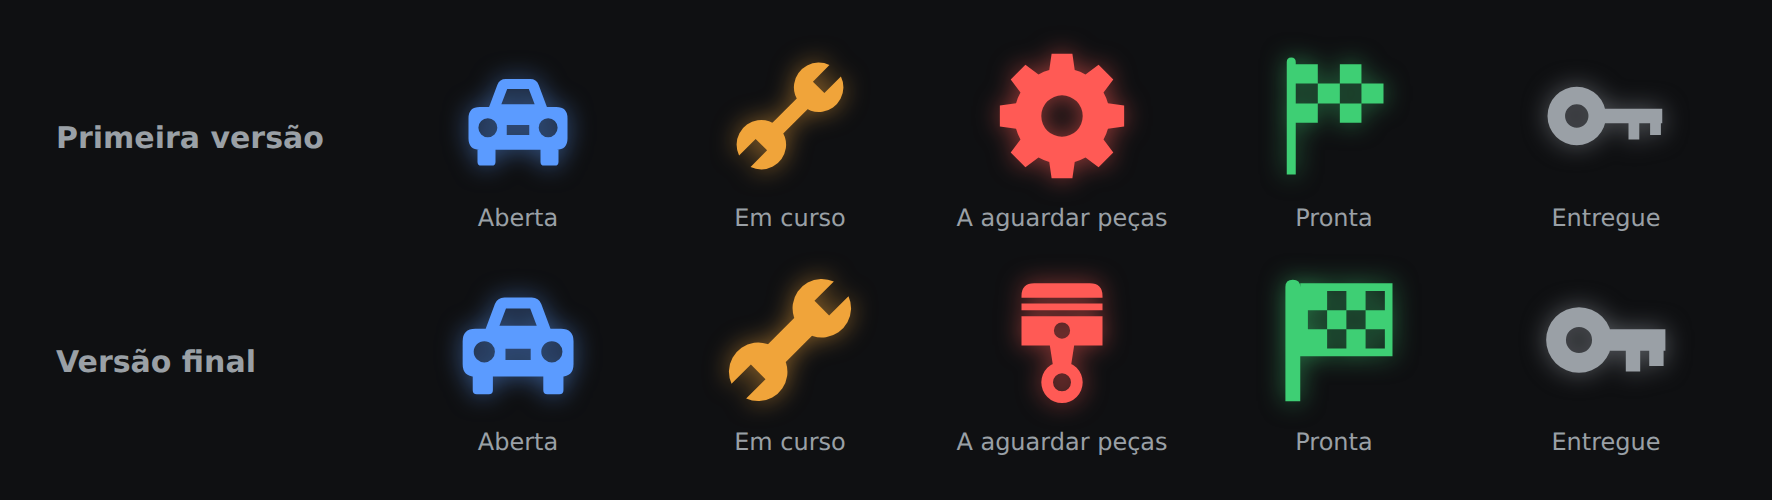
\includegraphics[width=\textwidth]{ferramentas/pictogramas.png}
  \caption[Os pictogramas antes e depois da revisão de design.]{Os pictogramas dos estados antes e depois da segunda passagem do revisor. ``A aguardar peças'' deixou de ser uma roda dentada, e a chave de bocas, a bandeira e a chave ficaram mais cheias, para as cinco luzes terem um peso visual parecido.}
  \label{fig:pictogramas}
\end{figure}

\subsection{taste-skill}

\begin{ficha}{taste-skill}{\texttt{Leonxlnx/taste-skill}}
  \item[O que é] Um conjunto de três \textit{skills} com regras para interfaces que não pareçam feitas em série por IA:
  \begin{itemize}
    \item \texttt{design-taste-frontend}, com as regras gerais;
    \item \texttt{redesign-existing-projects}, para melhorar um projeto que já existe;
    \item \texttt{stitch-design-taste}, para escrever o \texttt{DESIGN.md} num formato que outros agentes percebam.
  \end{itemize}
  \item[Para que serviu] As regras aplicadas na interface foram estas:
  \begin{itemize}
    \item um só acento de cor (o âmbar);
    \item fontes servidas pela própria aplicação;
    \item todos os estados de cada ecrã (a carregar, vazio, erro e normal);
    \item nada de ícones genéricos desenhados à mão (os pictogramas das luzes são próprios e pensados, o que é diferente);
    \item nenhum travessão nos textos da interface.
  \end{itemize}
  A parte de \textit{redesign} levou a analisar primeiro o que existia (o ecrã de entrada de julho) antes de mudar: foi daí que ficou a luz indicadora.
  \item[Porquê] Pedi-a pelo nome. Complementa a impeccable: a impeccable dá o processo, a taste-skill dá regras concretas contra o aspeto genérico.
  \item[Onde está] \texttt{.claude/skills/design-taste-frontend/}, \texttt{.claude/skills/redesign-existing-projects/}, \texttt{.claude/skills/stitch-design-taste/}.
\end{ficha}

\subsection{awesome-design-md e o formato DESIGN.md}

\begin{ficha}{awesome-design-md}{\texttt{VoltAgent/awesome-design-md}}
  \item[O que é] Uma coleção de ficheiros \texttt{DESIGN.md} inspirados nos sistemas visuais de produtos conhecidos.
  \item[Para que serviu] Referência de formato: como outros projetos organizam as cores, a tipografia, os componentes e as regras num \texttt{DESIGN.md}. Nenhum sistema visual de marca foi copiado: o da Bancada vem da oficina e da identidade que já tinha.
  \item[Porquê] Pedi-a pelo nome. Ver exemplos reais ajudou a escrever um \texttt{DESIGN.md} completo e no formato que as ferramentas esperam.
  \item[Onde está] Foi consultada, mas não faz parte do repositório.
\end{ficha}

\begin{ficha}{Formato DESIGN.md}{especificação da Google Labs}
  \item[O que é] Um formato para descrever um sistema visual: um bloco YAML com os \textit{tokens} (cores, tipografia, raios, espaços, componentes), seguido de oito secções em texto.
  \item[Para que serviu] O \texttt{DESIGN.md} da Bancada, com o sistema visual ``O Tablier da Oficina'', as regras com nome (por exemplo, ``A Regra da Voz Única'': o âmbar é a única cor de ação) e o que fazer e não fazer. O ficheiro \texttt{.impeccable/design.json} acrescenta o que o formato não guarda: rampas de cor, movimento e exemplos de componentes.
  \item[Porquê] Um sistema visual escrito deixa de depender da memória de quem o fez. Qualquer pessoa, ou agente de IA, que acrescente um ecrã tem as regras e os valores exatos à mão.
  \item[Onde está] \texttt{DESIGN.md}, \texttt{.impeccable/design.json}.
\end{ficha}

% ------------------------------------------------------------------
\section{Documentação e relatório}

\subsection{Documentos em Markdown}

A Tabela~\ref{tab:documentos} resume os documentos do repositório. Três deles (\texttt{AI.md}, \texttt{CLAUDE.md} e \texttt{AGENTS.md}) existem a pensar em agentes de IA. Um agente que abra o repositório pela primeira vez, ou uma sessão que foi compactada, recupera assim o contexto sem ter de o adivinhar.

\begin{table}[htbp]
\centering
\small
\begin{tabularx}{\textwidth}{@{}p{3.2cm}L@{}}
\toprule
\textbf{Documento} & \textbf{Para quê} \\
\midrule
\texttt{README.md} & apresentação do projeto, como o pôr a correr, estado, documentação e fluxo de trabalho \\
\texttt{PRODUCT.md} & o produto: utilizadores, problema, percurso de um carro pela oficina, o que existe e o que não existe (também lido pela impeccable) \\
\texttt{DESIGN.md} & o sistema visual, com os \textit{tokens} e as regras \\
\texttt{AI.md} & mapa do código para agentes de IA e pessoas: regras que não se podem partir, API, comandos, glossário \\
\texttt{CLAUDE.md} & memória do projeto para o Claude Code: preferências do autor, decisões tomadas, ambiente, estado atual e registo por data \\
\texttt{AGENTS.md} & ponto de entrada para outros agentes (aponta para o \texttt{AI.md} e o \texttt{CLAUDE.md}) \\
\texttt{docs/analise.md} & a revisão de segurança, desempenho e viabilidade \\
\bottomrule
\end{tabularx}
\caption{Os documentos do repositório.}
\label{tab:documentos}
\end{table}

\subsection{Ferramentas do relatório}

\begin{ficha}{LaTeX (TeX Live e latexmk)}{TeX Live 2023, latexmk 4.83}
  \item[O que é] Um sistema de composição de documentos a partir de texto com marcação.
  \item[Para que serviu] O relatório do projeto e este documento. Pacotes usados:
  \begin{itemize}
    \item \texttt{babel}, para o português;
    \item \texttt{booktabs} e \texttt{tabularx}, para as tabelas;
    \item \texttt{listings}, para o código;
    \item \texttt{dirtree}, para a árvore do repositório;
    \item \texttt{acronym}, para os acrónimos;
    \item \texttt{hyperref}, para as ligações;
    \item TikZ, para os dois diagramas deste documento, desenhados com as cores da Bancada.
  \end{itemize}
  O \texttt{latexmk} repete a compilação até as referências cruzadas estarem certas.
  \item[Porquê] O relatório já era em LaTeX desde a primeira fase. A composição tipográfica é melhor do que num processador de texto, e as referências a figuras, tabelas e secções atualizam-se sozinhas. O texto fonte fica no git, com histórico.
  \item[Onde está] \texttt{Relatorio/*.tex} e os PDF compilados ao lado.
\end{ficha}

\begin{ficha}{Graphviz}{2.43.0}
  \item[O que é] Desenho de diagramas a partir de uma descrição em texto (linguagem DOT).
  \item[Para que serviu] O esquema da base de dados da segunda versão e o diagrama da arquitetura, no relatório do projeto.
  \item[Porquê] Os diagramas da primeira versão foram feitos no ERDPlus e ficaram como imagens, e na revisão da terceira fase foram encontrados neles dois erros. Com o Graphviz, o diagrama é texto: fica no git ao lado do esquema, revê-se como código e volta a desenhar-se com um comando quando o esquema muda.
  \item[Onde está] \texttt{Relatorio/Anexos/*.dot}, com os PDF gerados ao lado.
\end{ficha}

\begin{ficha}{poppler-utils}{24.02.0}
  \item[O que é] Ferramentas de linha de comandos para PDF (\texttt{pdfinfo}, \texttt{pdftoppm}).
  \item[Para que serviu] Converter as páginas dos relatórios em imagens, para rever a paginação uma a uma: páginas quase vazias, figuras longe do texto, títulos sozinhos no fim de uma página.
  \item[Porquê] Um relatório que compila sem erros ainda pode ter má paginação, e isso só se vê a olhar para as páginas.
  \item[Onde está] Não deixa ficheiros no repositório: serve só para rever.
\end{ficha}

\begin{ficha}{Git e GitHub}{git 2.43.0}
  \item[O que é] Controlo de versões e o serviço onde o repositório está alojado.
  \item[Para que serviu]
  \begin{itemize}
    \item \textbf{Ramos}: o \texttt{main} é a versão estável, o \texttt{dev} a integração, e cada tarefa tem um ramo próprio.
    \item \textbf{Commits} em português, a explicar o porquê de cada mudança.
    \item \textbf{\textit{Pull requests}}: o da terceira fase entrou no \texttt{dev} com o CI verde.
  \end{itemize}
  \item[Porquê] Usei o GitHub desde o início. O ramo \texttt{dev} foi criado na terceira fase, a meu pedido, para haver mais organização: o que está no \texttt{main} só muda quando o \texttt{dev} está verificado.
  \item[Onde está] \url{https://github.com/TiagoPereira001/Projeto_final_UBI}.
\end{ficha}

% ------------------------------------------------------------------
\section{O assistente de programação: Claude Code}

\subsection{O que é e porque foi usado}

O Claude Code é um assistente de programação com inteligência artificial, da Anthropic. Trabalha diretamente num repositório: lê e escreve ficheiros, corre comandos num terminal, usa um browser e fala com o GitHub. Neste projeto correu num container na nuvem, com o repositório, o Node.js, o Docker e um Chromium instalados.

Usei-o na terceira fase porque o que pedi era grande e tinha pouco tempo:
\begin{itemize}
  \item uma análise profunda de segurança, desempenho e viabilidade;
  \item transformar o projeto numa plataforma para qualquer oficina;
  \item refazer a interface com o melhor design possível;
  \item criar os documentos de design e o mapa para agentes;
  \item rever o README e atualizar o relatório.
\end{itemize}
Um assistente que consegue ler o repositório inteiro, pôr o SQL Server a correr, escrever testes e ver a interface num browser consegue fazer isso e provar que funciona. As decisões de produto continuaram a ser minhas (secção~\ref{sec:decisoes}).

\subsection{Como trabalhou}

O trabalho seguiu sempre o mesmo ciclo (Figura~\ref{fig:fluxo}): ler e planear, alterar, testar, ver a interface no browser, rever o design, guardar e integrar. Nada era dado por feito sem passar pelas verificações.

\begin{figure}[htbp]
  \centering
  \setlength{\alturacorpo}{1.6cm}
  \begin{tikzpicture}[node distance=1cm and 0.62cm]
    \node[passo] (f1) {\passo{1. Pedido}{decisões do autor em perguntas estruturadas}};
    \node[passo, right=of f1] (f2) {\passo{2. Ler e planear}{Read, \texttt{grep}, lista de tarefas}};
    \node[passo, right=of f2] (f3) {\passo{3. Alterar}{Write, Edit, scripts em Python}};
    \node[passo, right=of f3] (f4) {\passo{4. Testar}{\texttt{node:test} e SQL Server, oxlint, \texttt{vite build}}};
    \node[passo, below=of f4] (f5) {\passo{5. Browser}{ver a interface: Playwright e Chromium, CSP, capturas}};
    \node[passo, left=of f5] (f6) {\passo{6. Rever design}{\texttt{impeccable detect}, revisor (segundo agente)}};
    \node[passo, left=of f6] (f7) {\passo{7. Guardar}{\texttt{git commit} em português, \texttt{git push}}};
    \node[passo, left=of f7] (f8) {\passo{8. Integrar}{\textit{pull request}, GitHub Actions e GitGuardian, merge no \texttt{dev}}};
    \draw[seta] (f1.text split east) -- (f2.text split west);
    \draw[seta] (f2.text split east) -- (f3.text split west);
    \draw[seta] (f3.text split east) -- (f4.text split west);
    \draw[seta] (f4.south) -- (f5.north);
    \draw[seta] (f5.text split west) -- (f6.text split east);
    \draw[seta] (f6.text split west) -- (f7.text split east);
    \draw[seta] (f7.text split west) -- (f8.text split east);
  \end{tikzpicture}
  \caption[O ciclo de trabalho da terceira fase.]{O ciclo de trabalho da terceira fase, com as ferramentas de cada passo, pela ordem dos números. Quando um dos passos de 4 a 8 falha, o trabalho volta ao passo 3.}
  \label{fig:fluxo}
\end{figure}

\subsection{As ferramentas do assistente}

O Claude Code tem ferramentas próprias, que usa para agir no repositório. A Tabela~\ref{tab:ferramentas-assistente} mostra as que foram usadas e quantas vezes. As contagens foram feitas com um script sobre o registo da sessão de trabalho, desde o primeiro pedido, a 26 de setembro de 2026, até ao pedido deste documento, a 27 de setembro. No total foram 510 chamadas.

\begin{table}[htbp]
\centering
\small
\begin{tabularx}{\textwidth}{@{}p{4.2cm}rL@{}}
\toprule
\textbf{Ferramenta} & \textbf{Vezes} & \textbf{Para quê} \\
\midrule
Bash (terminal) & 267 & correr testes, compilar, Docker, Playwright, git, scripts em Python, LaTeX, Graphviz \\
Write (escrever ficheiros) & 98 & criar ficheiros novos ou reescrever ficheiros inteiros \\
Read (ler ficheiros) & 66 & ler código, documentos, imagens das capturas e páginas dos PDF \\
Edit (editar ficheiros) & 10 & alterações pontuais (a maior parte das pontuais foi feita com scripts em Python) \\
TaskCreate e TaskUpdate & 12 e 22 & lista de tarefas visível, com o estado de cada uma \\
AskUserQuestion & 2 & as duas rondas de perguntas de decisão ao autor \\
Agent e SendMessage & 1 e 3 & o revisor de design: criado uma vez, retomado três vezes \\
ToolSearch & 6 & carregar ferramentas que só são ativadas quando são precisas \\
Ferramentas do GitHub & 15 & abrir o \textit{pull request}, ler o estado do CI e fazer o merge no \texttt{dev} (a tentativa de ativar o merge automático falhou, porque essa opção não está ligada no repositório) \\
Avisos e agendamento & 8 & subscrever e deixar de subscrever os eventos do \textit{pull request}, lê-los (4 vezes), agendar uma verificação e cancelá-la \\
\bottomrule
\end{tabularx}
\caption{As ferramentas do Claude Code usadas na terceira fase.}
\label{tab:ferramentas-assistente}
\end{table}

Dentro do terminal, estas foram as ferramentas que entraram em mais comandos:
\begin{itemize}
  \item scripts em Python (63 comandos) e o \texttt{git} (44);
  \item scripts do Playwright (28 comandos, 8 deles com o percurso completo da aplicação);
  \item o Docker (19) e as ferramentas de PDF do poppler (14);
  \item a compilação e o \textit{linter} do frontend (13 e 12);
  \item o \texttt{latexmk} (12), o Graphviz (11) e o \texttt{curl} (11);
  \item a linha de comandos da impeccable (12 chamadas, em 9 comandos);
  \item os testes da API (9).
\end{itemize}
Um comando pode usar várias ferramentas ao mesmo tempo.

\subsection{Ferramentas auxiliares}

\begin{itemize}
  \item \textbf{Python 3 (3.11), com PyYAML.} Serviu para alterações em muitos ficheiros de uma vez e para gerar ficheiros:
  \begin{itemize}
    \item pôr as regras de \texttt{:hover} dentro de \texttt{@media (hover: hover)} em todas as folhas de estilo;
    \item calcular a geometria dos pictogramas;
    \item gerar o \texttt{.impeccable/design.json} a partir do \texttt{DESIGN.md}, com rampas de cor em OKLCH;
    \item contar os números deste documento no registo da sessão.
  \end{itemize}
  Um script faz a mesma alteração em todo o lado e pode ser repetido.
  \item \textbf{curl.} Confirmar que a API estava de pé (\texttt{/api/saude}) antes de cada percurso no browser.
  \item \textbf{openssl.} Gerar passwords aleatórias para o SQL Server do CI e para os testes locais.
  \item \textbf{Docker (linha de comandos).} Arrancar, parar e apagar os SQL Server de desenvolvimento e de teste. No container na nuvem foi preciso arrancar o próprio serviço do Docker.
\end{itemize}

\subsection{Quem decidiu o quê}

A Tabela~\ref{tab:quem} separa o que foi decidido por mim do que foi feito pelo assistente na terceira fase. O código que ele escreveu passou pelos testes e pelo CI antes de entrar no \texttt{dev}.

\begin{table}[htbp]
\centering
\small
\begin{tabularx}{\textwidth}{@{}LL@{}}
\toprule
\textbf{Decidido por mim} & \textbf{Feito pelo assistente} \\
\midrule
\begin{itemize}[leftmargin=*,nosep,before=\vspace{-\baselineskip}]
  \item o nome Bancada;
  \item tornar o projeto geral, com a Duarte \& Raposo como primeiro cliente;
  \item manter e elevar a identidade visual;
  \item o registo público de oficinas;
  \item o tablet partilhado como dispositivo principal;
  \item o tablier como ecrã principal;
  \item usar a impeccable, a taste-skill e a awesome-design-md;
  \item criar o ramo \texttt{dev}, o \texttt{DESIGN.md}, o \texttt{AI.md}, o \texttt{CLAUDE.md} e o \texttt{PRODUCT.md};
  \item o relatório só com o que está feito;
  \item o merge automático para o \texttt{dev} com o CI verde.
\end{itemize}
&
\begin{itemize}[leftmargin=*,nosep,before=\vspace{-\baselineskip}]
  \item a revisão de segurança, desempenho e viabilidade;
  \item a segunda versão da base de dados e a API multi-oficina;
  \item os 52 testes e o CI;
  \item a interface nova e as correções pedidas pelo revisor;
  \item os documentos, os diagramas e as capturas;
  \item a atualização do relatório;
  \item o \textit{pull request}, o acompanhamento do CI e o merge.
\end{itemize}
\\
\bottomrule
\end{tabularx}
\caption{O que foi decidido pelo autor e o que foi feito pelo assistente na terceira fase.}
\label{tab:quem}
\end{table}

\subsection{Erros apanhados pelas verificações}

O assistente também se engana, e é por isso que cada passo tem uma verificação. A Tabela~\ref{tab:erros} mostra alguns dos erros apanhados durante a terceira fase e a verificação que os apanhou.

\begin{table}[htbp]
\centering
\small
\begin{tabularx}{\textwidth}{@{}Lp{3.1cm}@{}}
\toprule
\textbf{Erro} & \textbf{Apanhado por} \\
\midrule
Os índices únicos filtrados falhavam por falta de \texttt{SET QUOTED\_IDENTIFIER ON} no início do esquema. & criação da base de dados \\
Um teste usava \texttt{123456789} como exemplo de NIF inválido, mas esse número tem o dígito de controlo certo. & testes automáticos \\
Os botões só com ícone ficavam com largura zero, por causa de uma regra CSS para imagens. & percurso no browser \\
Os ícones Phosphor pesavam mais do dobro do código da aplicação. & medição do pacote \\
Os pontos do PIN tinham um brilho âmbar à volta, um efeito típico das interfaces geradas por IA. & detetor da impeccable \\
No tema escuro, a borda dos campos tinha um contraste de 2,7:1, abaixo do mínimo de 3:1. & script de contraste \\
Uma chamada ao \texttt{fetch} com opções inválidas. & oxlint \\
Um teste de segurança dava falso positivo porque o nome da oficina de teste continha a palavra ``Hashes''. & testes automáticos \\
As luzes do tablier estavam dentro de lentes e pareciam botões. & revisor de design (1.ª passagem) \\
A animação de arranque das luzes repetia sempre que se voltava ao quadro. & revisor de design (2.ª passagem) \\
A roda dentada de ``a aguardar peças'' confundia-se com ``Definições''. & revisor de design (2.ª passagem) \\
O Graphviz trocava as marcas das ligações entre tabelas lado a lado. & revisão das páginas do PDF \\
\bottomrule
\end{tabularx}
\caption{Alguns erros da terceira fase e a verificação que os apanhou.}
\label{tab:erros}
\end{table}

\subsection{Limites e transparência}

\begin{itemize}
  \item \textbf{O assistente não substitui o teste com utilizadores reais.} A aplicação ainda não foi usada pelos mecânicos da Duarte \& Raposo.
  \item \textbf{O veredito final do revisor de design (``ship'') tem um âmbito limitado.} Cobre as correções que foram pontuadas na última passagem, e não é uma aprovação nova de toda a interface.
  \item \textbf{Os dados das capturas e da demonstração são fictícios.} Os segredos do projeto (as passwords da base de dados e o segredo das sessões) nunca foram escritos no repositório.
  \item \textbf{O uso do Claude Code e das skills de design está declarado} na secção 4.5 do relatório do projeto e neste documento. As regras da UBI sobre o uso de IA em trabalhos académicos devem ser confirmadas por mim antes da entrega.
\end{itemize}

% ------------------------------------------------------------------
\section{Ferramentas das duas primeiras fases}

As duas primeiras fases foram desenvolvidas no meu computador, com Arch Linux, onde também corria o SQL Server em Docker.

\begin{ficha}{Visual Studio Code}{editor}
  \item[O que é] Um editor de código.
  \item[Para que serviu] Escrever a base de dados, a API e o início da interface nas duas primeiras fases. A extensão SQL Server serviu para confirmar a ligação à base de dados e ver as tabelas.
  \item[Porquê] É o editor que uso no curso, com extensões para JavaScript, React, Docker e SQL.
  \item[Onde está] O ficheiro de \textit{workspace} esteve no repositório em julho.
\end{ficha}

\begin{ficha}{Thunder Client e curl}{testes manuais}
  \item[O que é] Um cliente HTTP dentro do VS Code (semelhante ao Postman) e a ferramenta de linha de comandos para pedidos HTTP.
  \item[Para que serviu] Os testes manuais da primeira API: criar e listar clientes, recusar autocaravanas de clientes inexistentes ou com matrícula repetida, confirmar que a password não aparecia nas respostas.
  \item[Porquê] Eram a forma mais rápida de testar rota a rota enquanto a API crescia. Na terceira fase, estes cenários passaram para os testes automáticos.
  \item[Onde está] Os cenários estão na Tabela 5 do relatório do projeto.
\end{ficha}

\begin{ficha}{ERDPlus}{diagramas}
  \item[O que é] Uma ferramenta web para diagramas entidade-relação e esquemas relacionais.
  \item[Para que serviu] O diagrama concetual e o esquema relacional da primeira versão.
  \item[Porquê] É simples e segue a notação usada nas aulas. Os dois erros que os diagramas tinham estão explicados no relatório. Na segunda versão, os diagramas passaram para o Graphviz.
  \item[Onde está] \texttt{Relatorio/Anexos/Diagrama.png}, \texttt{Relatorio/Anexos/Esquema\_relacional.png}.
\end{ficha}

As outras ferramentas das primeiras fases (Docker, SQL Server, Node.js, Express, React, Vite, GitHub e LaTeX) continuaram na terceira fase e estão descritas nas secções anteriores.

% ------------------------------------------------------------------
\section{Conclusão}

As ferramentas da Bancada dividem-se em dois grupos. As da aplicação foram, na maior parte, escolhidas por mim nas primeiras fases e mantiveram-se: SQL Server, Node.js, Express, React, Vite e Docker. O que mudou nelas foi a forma de as usar: sessões em cookies, CSP rigorosa, porta do SQL Server só local, permissões mínimas, menos dependências.

As ferramentas novas da terceira fase servem sobretudo para duas coisas. A primeira é provar que o sistema funciona: testes contra um SQL Server real, integração contínua, percursos num browser a sério e um revisor de design independente. A segunda é deixar o conhecimento escrito: o \texttt{DESIGN.md}, o \texttt{PRODUCT.md}, o \texttt{AI.md}, o \texttt{CLAUDE.md} e os diagramas em texto. O assistente de IA fez grande parte do trabalho desta fase, mas as decisões de produto foram minhas, e o código que ele escreveu passou pelos mesmos testes e pela mesma integração contínua.

A Tabela~\ref{tab:resumo} resume cada ferramenta numa frase.

\small
\begin{xltabular}{\textwidth}{@{}>{\raggedright\arraybackslash}p{3.5cm}>{\raggedright\arraybackslash}p{2.8cm}L@{}}
\caption{Cada ferramenta numa frase.}\label{tab:resumo}\\
\toprule
\textbf{Ferramenta} & \textbf{Área} & \textbf{Porquê, numa frase} \\
\midrule
\endfirsthead
\toprule
\textbf{Ferramenta} & \textbf{Área} & \textbf{Porquê, numa frase} \\
\midrule
\endhead
\bottomrule
\endfoot
SQL Server 2022 & base de dados & já escolhido e testado, e garante na própria BD as regras mais importantes \\
mssql & base de dados & \textit{pool} único e consultas parametrizadas \\
sqlcmd & base de dados & saber quando o SQL Server está pronto \\
Node.js 22 & API & versão LTS que substitui o nodemon, o dotenv e o Supertest \\
Express 5 & API & rotas e \textit{middleware}; as exceções assíncronas chegam ao tratamento de erros \\
jsonwebtoken e cookie-parser & API & sessão num cookie que o JavaScript não lê \\
bcrypt & API & passwords e PINs com um \textit{hash} lento e login de tempo constante \\
helmet & API & CSP rigorosa e cabeçalhos de segurança \\
express-rate-limit & API & limites por conta e por IP, sem bloquear a oficina inteira \\
compression & API & menos dados na rede do tablet \\
React 19 & interface & a biblioteca já escolhida, com componentes próprios \\
Vite 8 & interface & desenvolvimento rápido e compilação com páginas à parte \\
React Router 7 & interface & rotas e páginas de gestão carregadas só quando são precisas \\
vite-plugin-pwa & interface & instalável no tablet e abre logo \\
Fontsource (Barlow) & interface & fontes da própria aplicação, compatíveis com a CSP \\
Phosphor + gerador & interface & ícones só com os pesos usados (menos 22~KB) \\
Pictogramas SVG próprios & interface & luzes de aviso que parecem as de um carro \\
CSS com tokens & interface & um sistema visual próprio em 8,4~KB \\
Docker e Compose & infraestrutura & o mesmo ambiente em qualquer computador \\
Dockerfile em etapas & infraestrutura & imagem pequena, sem \texttt{root} \\
\texttt{.env} e \texttt{.env.example} & infraestrutura & segredos fora do código \\
node:test & qualidade & 52 testes contra um SQL Server real, sem dependências \\
oxlint & qualidade & \textit{linter} instantâneo \\
GitHub Actions & qualidade & nada entra no \texttt{dev} sem os testes passarem \\
npm audit e lockfiles & qualidade & dependências verificadas e iguais em todas as máquinas \\
GitGuardian & qualidade & procura segredos em cada \textit{pull request} \\
Playwright e Chromium & qualidade & ver a interface a funcionar, com capturas e medições \\
Script de contraste & qualidade & contraste do texto e das bordas confirmado nos dois temas \\
impeccable & design & processo com direção escrita, detetor e revisor independente \\
taste-skill & design & regras contra o aspeto genérico \\
awesome-design-md & design & exemplos do formato \texttt{DESIGN.md} \\
Formato DESIGN.md & design & o sistema visual escrito e reutilizável \\
Markdown (7 documentos) & documentação & contexto para pessoas e para agentes de IA \\
LaTeX e latexmk & relatório & composição de qualidade e texto fonte no git \\
Graphviz & relatório & diagramas como texto, fáceis de atualizar \\
poppler-utils & relatório & rever a paginação página a página \\
Git e GitHub & todos & ramos, \textit{pull requests} e histórico \\
Claude Code & desenvolvimento & a terceira fase, com decisões do autor e verificação em cada passo \\
Python, curl, openssl & desenvolvimento & alterações em lote, verificações e passwords aleatórias \\
VS Code, Thunder Client, ERDPlus & fases 1 e 2 & escrever, testar à mão e desenhar a primeira versão \\
\end{xltabular}
\normalsize

\clearpage

% ------------------------------------------------------------------
\section*{Anexo A: Versões usadas}
\addcontentsline{toc}{section}{Anexo A: Versões usadas}

\begin{table}[H]
\centering
\small
\begin{tabularx}{\textwidth}{@{}p{5cm}L@{}}
\toprule
\textbf{Ferramenta} & \textbf{Versão} \\
\midrule
Node.js e npm & 22.22.2 e 10.9.7 \\
SQL Server & 2022 (\texttt{mcr.microsoft.com/mssql/server:2022-latest}) \\
Express, mssql, bcrypt & 5.2.1, 12.7.2, 6.0.0 \\
helmet, express-rate-limit & 8.3.0, 8.7.0 \\
jsonwebtoken, cookie-parser, compression & 9.0.3, 1.4.7, 1.8.2 \\
React, React Router, Vite & 19.3.0, 7.18.4, 8.3.1 \\
vite-plugin-pwa, oxlint & 1.3.0, 1.85.0 \\
@fontsource/barlow, @phosphor-icons/core & 5.3.0, 2.1.1 \\
Docker, Docker Compose & 29.3.1, v5.1.1 \\
GitHub Actions & \texttt{actions/checkout@v7}, \texttt{actions/setup-node@v7} \\
Playwright, Chromium & 1.63.0, 141 \\
TeX Live, pdfTeX, latexmk & 2023, 1.40.25, 4.83 \\
Graphviz, poppler-utils & 2.43.0, 24.02.0 \\
Python, git & 3.11, 2.43.0 \\
\bottomrule
\end{tabularx}
\caption{Versões das ferramentas usadas na terceira fase.}
\label{tab:versoes}
\end{table}

\section*{Anexo B: Comandos principais}
\addcontentsline{toc}{section}{Anexo B: Comandos principais}

\begin{table}[H]
\centering
\small
\begin{tabularx}{\textwidth}{@{}p{6.4cm}L@{}}
\toprule
\textbf{Comando} & \textbf{O que faz} \\
\midrule
\texttt{docker compose up -d} & arranca o SQL Server (só em \texttt{127.0.0.1}) \\
\texttt{npm run db:setup} & cria a base de dados, as tabelas e o login da API \\
\texttt{npm run db:seed} & carrega a Duarte \& Raposo com dados fictícios \\
\texttt{npm run dev} (backend) & API em \texttt{http://localhost:3000} \\
\texttt{npm run dev} (frontend) & interface em \texttt{http://localhost:5173} \\
\texttt{npm test} (backend) & os 52 testes contra o SQL Server \\
\texttt{npm run lint \&\& npm run build} & \textit{linter} e compilação do frontend \\
\texttt{npm run icones} & gera o módulo de ícones só com os pesos usados \\
\texttt{docker compose -{}-profile app up -d -{}-build} & a aplicação completa em containers \\
\texttt{latexmk -pdf <ficheiro>.tex} & compila um relatório \\
\texttt{dot -Tpdf <ficheiro>.dot -o <ficheiro>.pdf} & desenha um diagrama \\
\bottomrule
\end{tabularx}
\caption{Comandos principais do projeto.}
\label{tab:comandos}
\end{table}

\end{document}
